\documentclass{article}
\usepackage[utf8]{inputenc}

\usepackage{xr}
\usepackage{amssymb}
\usepackage{amsmath}
\usepackage{amsthm}
\usepackage{subcaption}

\usepackage{pgf,tikz,tkz-graph}
\usetikzlibrary{arrows,shapes}

\usepackage{xspace} % A makrok utani space korrekt kezelese miatt.

\newcommand{\cl}[1]{\mbox{\ensuremath{\mathbf{#1}}}\xspace}
\renewcommand{\P}{\cl{P}}
\newcommand{\NP}{\cl{NP}}
\def\coNP{\cl{co}-\cl{NP}}
\newcommand{\N}{\mathbb{N}}
\newcommand{\R}{\mathbb{R}}
\newcommand{\rplus}{\mathbb{R}_{\ge 0}}
\newcommand{\Z}{\mathbb{Z}}
\newcommand{\Sphere}{\mathbb{S}}
%%%%%%%%%%%%%%%%%%%%%%%%%%%%%%%%%%%%%%%%%%%%%%%%%%%%%

\begin{document}

\begin{center}
	xy házija, 1. feladatsor
\end{center}

\paragraph{1.2 feladat}
Ide írom a megoldásomafiafnanfnfnfydadadjnadjanjd.
Lehet benne néhány képlet $\frac{1}{2}\sum_{i=1}^n x_i^j$.
Vagy kiemelt képlet $$\frac{1}{2}\sum_{i=1}^n x_i^j.$$
Több info itt: \verb|https://en.wikibooks.org/wiki/LaTeX/Mathematics|

\bigskip


Esetleg ábrát is lehet csinálni.

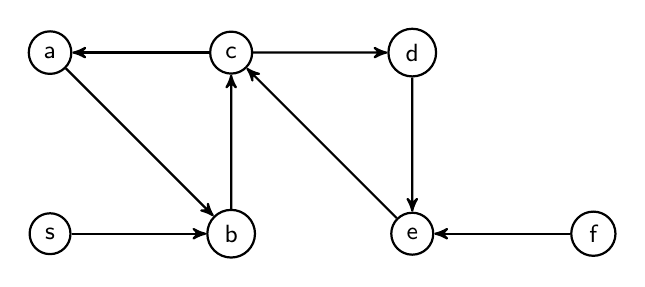
\begin{tikzpicture}[->,>=stealth',auto,scale=2.3,
thick,every node/.style={circle,draw,font=\sffamily\small}]

\node (s) at (0, 0) {s};
\node (a) at (0, 1) {a};
\node (b) at (1, 0) {b};
\node (c) at (1, 1) {c};
\node (d) at (2, 1) {d};
\node (e) at (2, 0) {e};
\node (f) at (3, 0) {f};
\path[every node/.style={font=\sffamily\small}]
(s) edge node {} (b)
(a) edge node {} (b)
(b) edge node {} (c)
(c) edge node {} (a)
(c) edge node {} (d)
(d) edge node {} (e)
(e) edge node {} (c)
(f) edge node {} (e);
\end{tikzpicture}


\bigskip
Vagy lehet rajzolni egyet pl geogebrában vagy paint-ben és beszúrni. Info itt: \verb|https://en.wikibooks.org/wiki/LaTeX/Importing_Graphics|.

\vspace{2cm}
Ez egy elég jó online editor: \verb|https://www.overleaf.com/|, de vannak offline editorok is, pl a TeXstudio.


\end{document}